
\section{Problem 5}
\label{part5}
\begin{verbatim}
----Extra Credit 5 points----
 Re-run question 2, but this time with proper TFIDF calculations
instead of the hack discussed on slide 7 (p. 32).  Use the same 500
words, but this time replace their frequency count with TFIDF scores
as computed in assignment #3.  Document the code, techniques,
methods, etc. used to generate these TFIDF values.  Upload the new
data file to github.

Compare and contrast the resulting dendrogram with the dendrogram
from question #2.

Note: ideally you would not reuse the same 500 terms and instead
come up with TFIDF scores for all the terms and then choose the top
500 from that list, but I'm trying to limit the amount of work
necessary.
\end{verbatim}

\subsection{Solution}
\begin{enumerate}
\item In this question I have to compute a blog matrix again but this time with the proper TFIDF calculations instead of the frequency of occurrences of the words.
\item For this I have used concept from previous assignment on how to calculate TFIDF.Words having TFIDF values are chosen to be in the matrix.
\item I have calculated TF value for each word with respect to each blog which is inturn used to calculate TF values.
\item  have used ``generatefeedvector.py'' again to generate the blog matrix and for generating the Dendogram I have used code from question 2.
\item My code for generating the blog matrix can be found in the listing\ref{lst:q5-1} and code for generating Dendogram and ASCII can be found in listing\ref{lst:q5-2}.
\item Sample blog data can be found in the fig\ref{Sample5_t1}.
\item Once I got the blog data I processed this data to be ASCII file and a Dendogram. This process is similar to the process in question 2.
\item Dendogram can be found in the fig\ref{graph51} and sample ASCII file can be found in the fig\ref{Sample5_t2}.
\item When compared to the Dendogram in the question 2, similarties for the ``F-Measure'' and ``Web Science'' have changed. 
\item In the previous Dendogram ``F-Measure'' is similar to ``Samtastic! Review'' and now it is similar to ``I/Love/Total/Distruction''.
\item In the previous Dendogram ``Web Science and Digital Library Research Group'' is similar to ``Mile In Mine'' and now it is similar to ``The Moon Topples''.
\item Comparitively number of clusters in the present Dendogram are more than the number of clusters in the Dendogram generated in question 2.
\item I have also observed that the almost all the clusters are around the same blogs but with different hierarchy.
\end{enumerate}
\newpage

\subsection{Code Listing}
\subsubsection{Code Listing 1}

\lstinputlisting[language=Python,breaklines = true,frame=single,caption={Python code for getting blog matrix using TFIDF scores}, label=lst:q5-1,captionpos=b,numbers=left,showspaces=false,showstringspaces=false,basicstyle=\footnotesize]{tfidf_gettingblogdata.py}
\newpage

\subsubsection{Code Listing 2}

\lstinputlisting[language=Python,breaklines = true,frame=single,caption={Python code for getting dendogram}, label=lst:q5-2,captionpos=b,numbers=left,showspaces=false,showstringspaces=false,basicstyle=\footnotesize]{q5_2.py}
\newpage

\subsection{Outputs}
\subsubsection{Sample blog matrix}
\begin{figure}[ht]    
    \begin{center}
        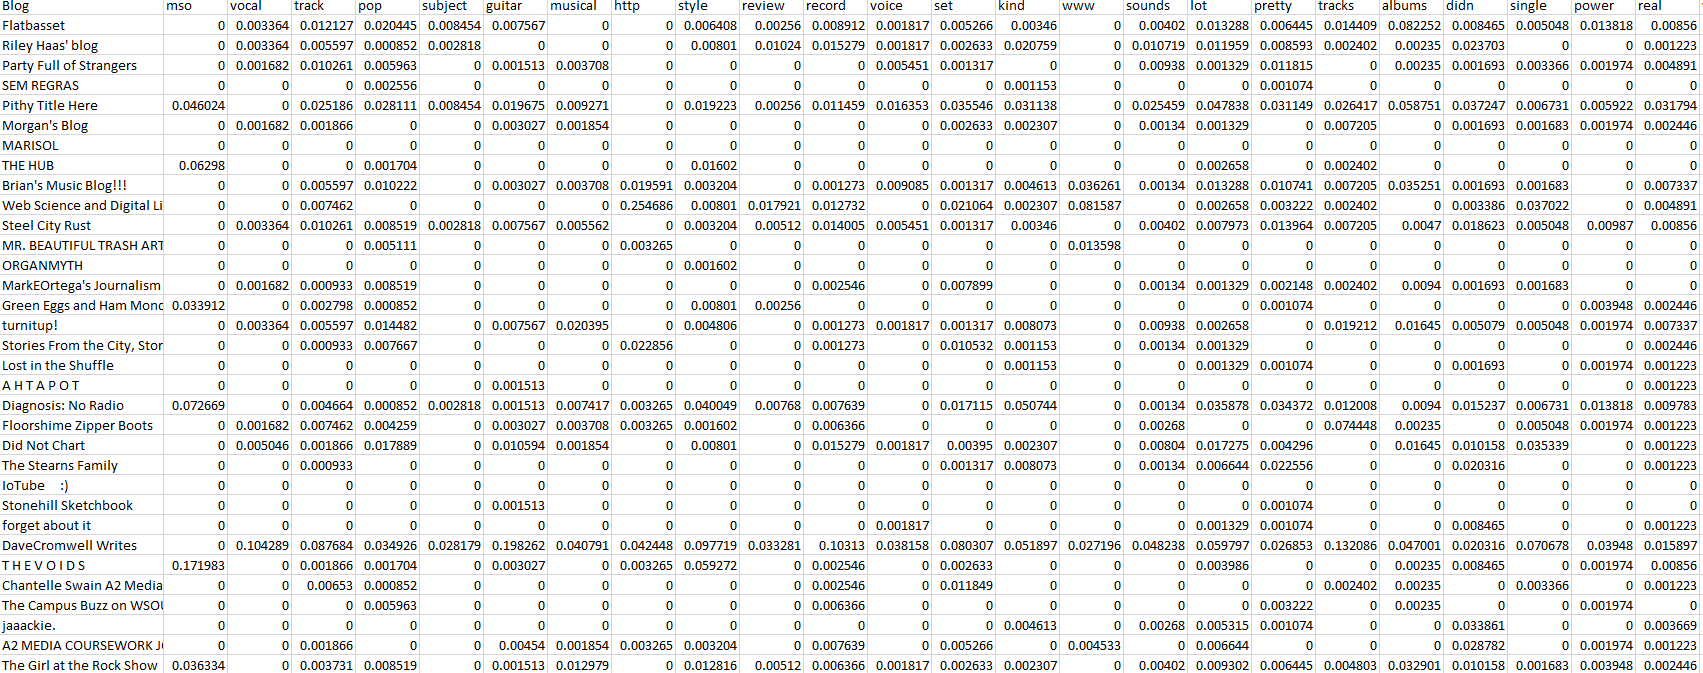
\includegraphics[scale=0.4]{sampletfidfblog.png}
        \caption{Sample blog matrix formed using TFIDF values}
        \label{Sample5_t1}
    \end{center}
\end{figure}
\newpage
\subsubsection{Sample ASCII file}
\begin{figure}[ht]    
    \begin{center}
        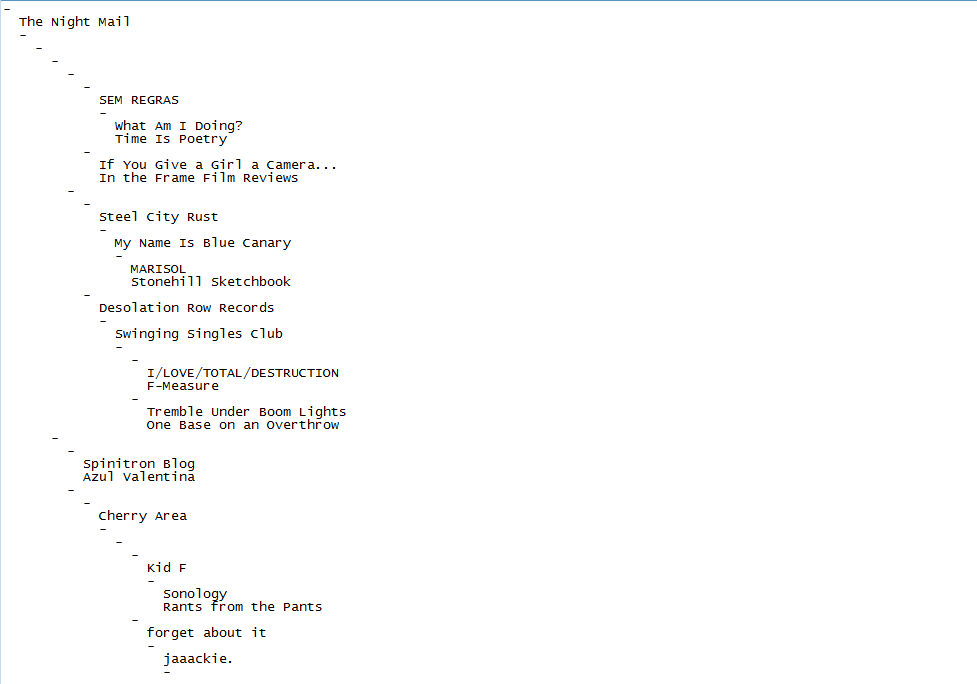
\includegraphics[scale=0.8]{sample_ascii5_2.png}
        \caption{Sample ASCII file showing clustering of most similar blogs }
        \label{Sample5_t2}
    \end{center}
\end{figure}
\newpage
\subsubsection{Dendogram}
\begin{figure}[ht]    
    \begin{center}
        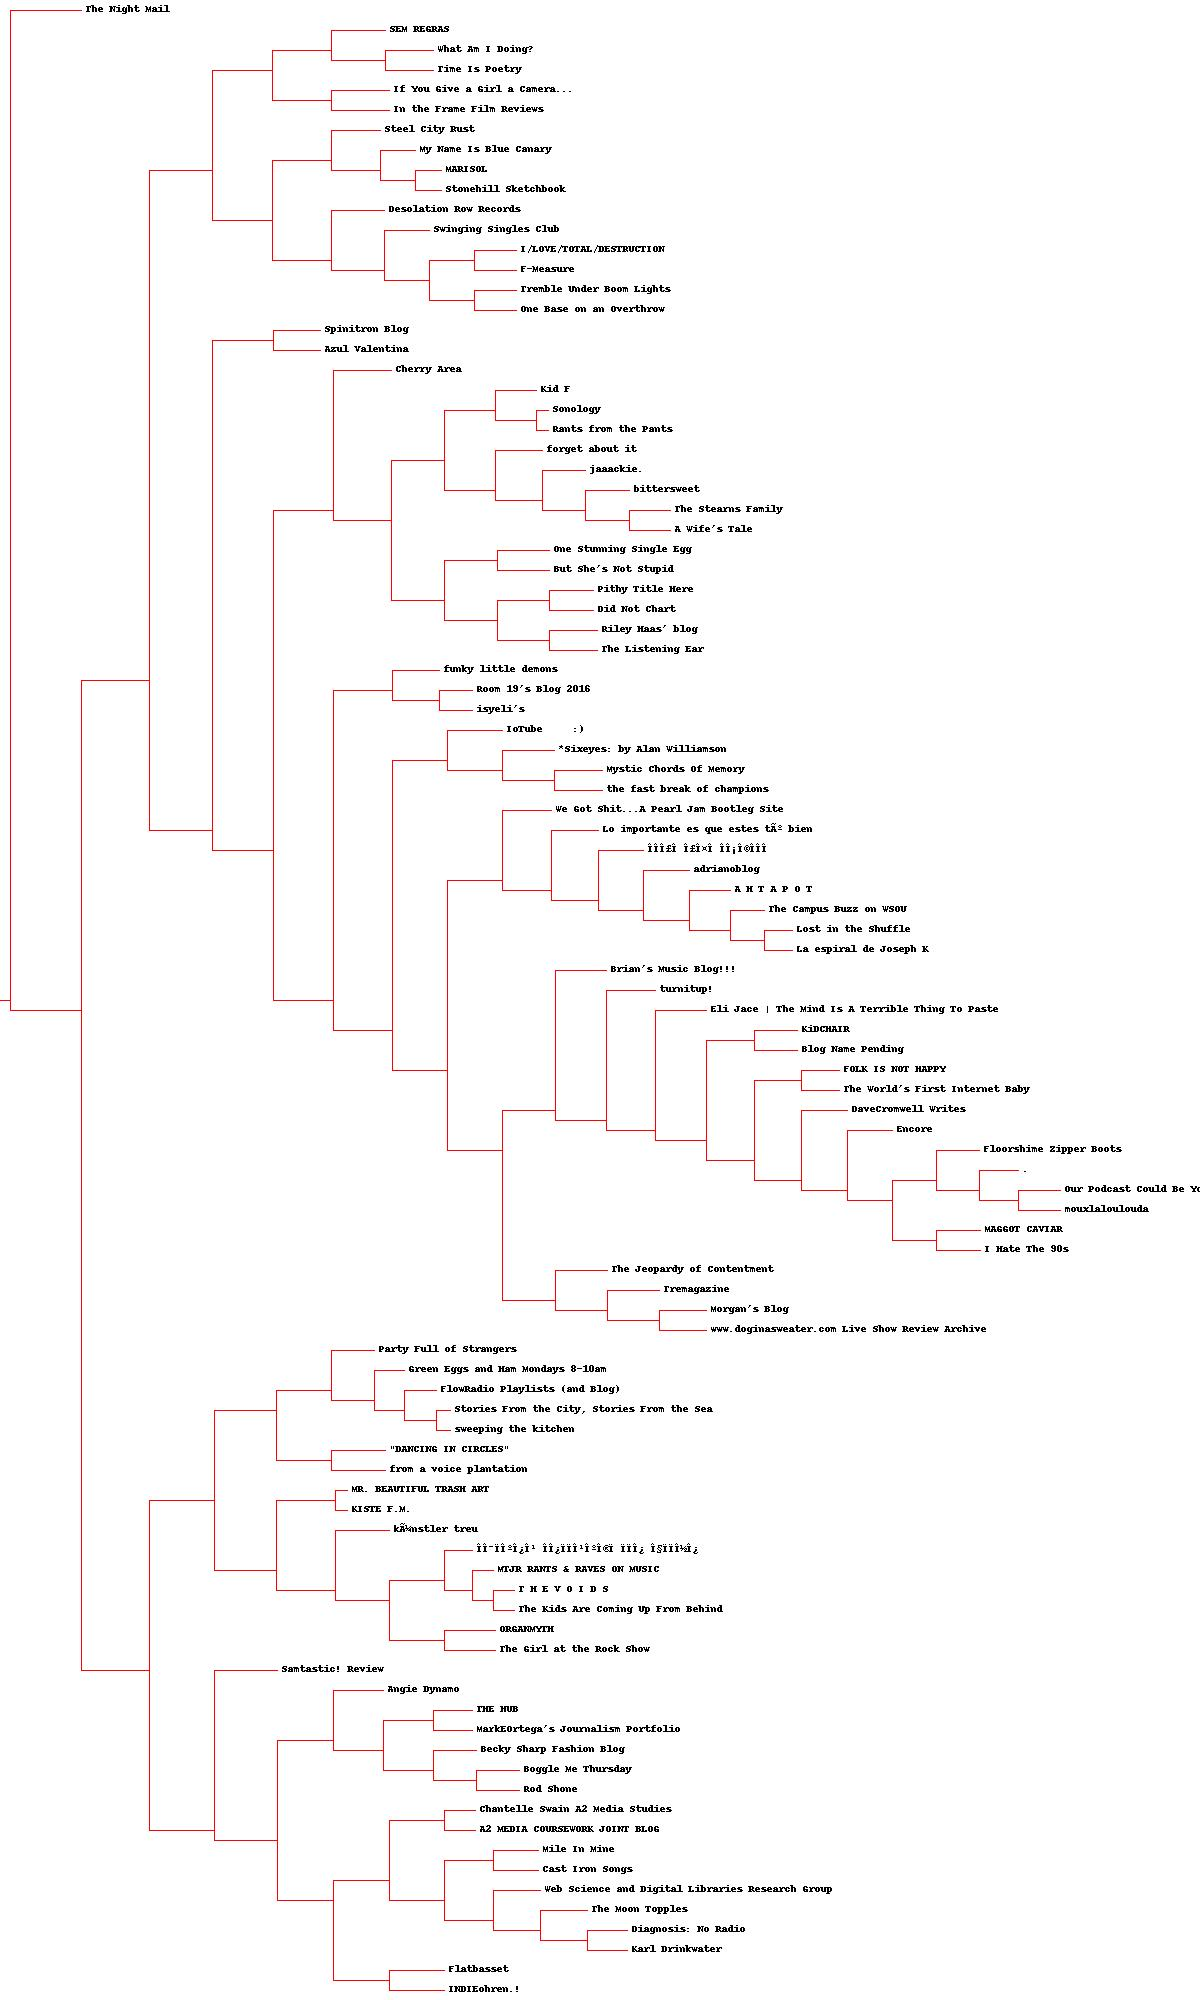
\includegraphics[scale=0.23]{clusterblogtfidf.jpg}
        \caption{Dendogram showing clustering of most similar blogs}
        \label{graph51}
    \end{center}
\end{figure}
\newpage
